\documentclass[9pt,letterpaper]{article}
% Some useful packages for including images, colored font, etc.
\usepackage{url}
\usepackage[yyyymmdd,hhmmss]{datetime}
\usepackage{pdfsync}
\usepackage{enumitem}
\usepackage{amsmath}
\usepackage{amssymb}
\usepackage{outline}
\usepackage{dsfont}
\usepackage{comment}
\usepackage{lmodern}
\usepackage{cite}
\usepackage{float}
\usepackage{appendix}
\usepackage{fancyvrb}
\usepackage{hyperref}

\usepackage{listings,xcolor}
\usepackage{courier}
\usepackage{textcomp}

\usepackage{graphicx}
\graphicspath{{./figures/}}
\graphicspath{{figures/}}

\bibliographystyle{unsrt}
\usepackage{fancyhdr}
\usepackage{datetime}
\fancyhf{}
\fancyhead[C]{\today\ DRAFT}
\pagestyle{fancy}

\newcommand{\stt}[1]{\begin{footnotesize}\texttt{#1}\end{footnotesize}}

\usepackage{makecell}      % cells in tables to handle multiline content (see Ch5)
\usepackage{hhline}

% Nice package! https://www.overleaf.com/learn/latex/Page_size_and_margins#Paper_size.2C_orientation_and_margins
\usepackage{geometry}
 \geometry{
%  a4paper,
%  total={170mm,257mm},
   left=30mm,
   right=30mm,
   top=25mm,
 }

 % ^^3f is a question mark (UTF-8)

% Begin JavaScript listinglst --------------------------------

\usepackage{color} %use color
\definecolor{mygreen}{rgb}{0,0.6,0}
\definecolor{myred}{rgb}{0.8,0.2,0.2}
\definecolor{mygray}{rgb}{0.5,0.5,0.5}
\definecolor{mymauve}{rgb}{0.58,0,0.82}

%Customize a bit the look
\lstset{ %
backgroundcolor=\color{white}, % choose the background color; you must add \usepackage{color} or \usepackage{xcolor}
basicstyle=\footnotesize, % the size of the fonts that are used for the code
breakatwhitespace=false, % sets if automatic breaks should only happen at whitespace
breaklines=true, % sets automatic line breaking
captionpos=b, % sets the caption-position to bottom
commentstyle=\color{mygreen}, % comment style
deletekeywords={...}, % if you want to delete keywords from the given language
escapeinside={\%*}{*)}, % if you want to add LaTeX within your code
extendedchars=true, % lets you use non-ASCII characters; for 8-bits encodings only, does not work with UTF-8
%pod frame=single, % adds a frame around the code
keepspaces=true, % keeps spaces in text, useful for keeping indentation of code (possibly needs columns=flexible)
keywordstyle=\color{blue}, % keyword style
% language=Octave, % the language of the code
morekeywords={*,...}, % if you want to add more keywords to the set
numbers=left, % where to put the line-numbers; possible values are (none, left, right)
numbersep=5pt, % how far the line-numbers are from the code
numberstyle=\tiny\color{mygray}, % the style that is used for the line-numbers
rulecolor=\color{black}, % if not set, the frame-color may be changed on line-breaks within not-black text (e.g. comments (green here))
showspaces=false, % show spaces everywhere adding particular underscores; it overrides 'showstringspaces'
showstringspaces=false, % underline spaces within strings only
showtabs=false, % show tabs within strings adding particular underscores
stepnumber=1, % the step between two line-numbers. If it's 1, each line will be numbered
stringstyle=\color{mymauve}, % string literal style
tabsize=2, % sets default tabsize to 2 spaces
title=\lstname % show the filename of files included with \lstinputlisting; also try caption instead of title
}
%END of listing package%

\definecolor{darkgray}{rgb}{.4,.4,.4}
\definecolor{purple}{rgb}{0.65, 0.12, 0.82}

%define Javascript language (modified for  RADmapper)
\lstdefinelanguage{JavaScript}{
  keywords={\$abs, \$append, \$assert, \$average, \$base64decode, \$base64encode, \$boolean, \$ceil, \$contains, \$count, \$decodeUrl, \$decodeUrlComponent, \$distinct, \$each, \$encodeUrl, \$encodeUrlComponent, \$error, \$eval, \$exists, \$filter, \$floor, \$formatBase, \$formatInteger, \$formatNumber, \$fromMillis, \$join, \$keys, \$length, \$lookup, \$lowercase, \$map, \$match, \$max, \$merge, \$millis, \$min, \$not, \$now, \$number, \$pad, \$parseInteger, \$power, \$random,,\$read, \$readSpreadsheet, \$reduce, \$replace, \$reverse, \$round, \$shuffle, \$sift, \$single, \$sort, \$split, \$spread, \$sqrt, \$string, \$substring, \$substringAfter, \$substringBefore, \$sum, \$toMillis, \$trim, \$type,,\$uppercase, \$zip},
keywordstyle=\color{darkgray}\bfseries,
ndkeywords={false, function, express, query, true}
ndkeywordstyle=\color{darkgray}\bfseries,
identifierstyle=\color{black},
sensitive=false,
morecomment=\bfseries[s]{/*}{*/},
commentstyle=\color{purple}\ttfamily,
stringstyle=\color{myred}\ttfamily,
morestring=[b]',
morestring=[b]"
}
% End JavaScript listinglst -------------------------------

\begin{document}
\title{Draft OAGi Interoperable Mapping Specification}
\author{OAGi Members}
\maketitle

\section{Introduction}
This document describes a data mapping language designed to serve as an \textit{interoperable exchange form} for expressing the intent of many mapping and data restructuring needs.
As an interoperable exchange form, it is intended that the language can be translated (by humans and machine agents) into mapping specification in other languages.
For example, it should be possible to translate statements in the exchange form into mapping specification used by commercial mapping tools.
%OAGi members can find the most recent version of this document in the \textit{OAGi Mapping Specification Working Group} Confluence pages (under ``Mapping Doc'').

The mapping language  described (provisionally called RADmapper) borrows predominantly from the JSONata language~\cite{Jsonata.org2021}, but also includes provisions for mapping to/from forms other than JSON.\@
These forms include tables (e.g. Excel) XML, and networks of data such as knowledge graphs.
The RADmapper language also addresses additional use cases, including in-place updating of target data sources, and mapping from multiple sources.
To support networks of data, the mapping language borrows ideas from the Object Management Group's Queries, Views and Transformation relational (QVT-r)~\cite{ObjectManagementGroup2016b} mapping language, and Datalog~\cite{Abiteboul1995a}.

The document describes the RADmapper language and the concept behind how it is can be transformed to an interoperable exchange form.
As of this writing, the canonical form of the interoperable exchange form is under development.
A reference implementation of the RADmapper language can be found in \href{https://github.com/pdenno/RADmapper}{this GitHub repository}.
The document is a draft and as of this writing (\today) is likely to be updated often.
%Whether or not the tool is useful for transforming information in real-world settings remains to be seen;
%we'll generate an OpenAPI Specification for the tool to test that idea.

% Discussion of the AST idea and the role of "RADmapper language" in that.

% At the current state of development, it isn't clear whether the language being described is the interoperable exchange form itself or something derived from the executable language being developed.
% For example, it is possible that abstract syntax trees (ASTs) of content in the language being described could themselves be transformed
% into the actual exchange form.
%The same process could possibly be used to produce ``mapping tables'', spreadsheets provided to programmers to hand-code the transformations
%in their system's native programming language. %A diagram would help here.
%In this light, the RADmapper tool can be thought of as means to get the intent of the mapping correct before handing it off to programmers.
% But this discussion is getting ahead of itself; the next section surveys key aspects of the language.

\section{Quick Start: Example Mapping Tasks}

This section uses examples to describe the basic features of the RADmapper language.
RADmapper provides the complete expression language and all the built-in functions of JSONata; therefore the examples focus on the new concepts not in JSONata.
Examples of JSONata can be found in the \href{https://jsonata.org/}{JSONata specification}.

\subsection{Simple Restructuring}

This example illustrates simple restructuring of a data structure.
The example is based on a discussion on the JSONata Slack channel.
The goal of the example is to swap the nesting of \stt{owners} and \stt{systems} as shown in Figure~\ref{data:simple-restructuring}.

\begin{figure}[H]
  \caption{The goal is to swap the nesting of 'owners' and 'systems' in the data on Lines 1--9
  so that it looks Lines 13--21.}
 \label{data:simple-restructuring}
\begin{lstlisting}[language=JavaScript,basicstyle=\ttfamily\scriptsize,numberstyle=\scriptsize]
{ "systems":
   { "system1": { "owners": { "owner1": { "device1": { "id": 100, "status": "Ok" },
                                          "device2": { "id": 200, "status": "Ok" }},
                              "owner2": { "device3": { "id": 300, "status": "Ok" },
                                          "device4": { "id": 400, "status": "Ok" }}}},
     "system2": { "owners": { "owner1": { "device5": { "id": 500, "status": "Ok" },
                                          "device6": { "id": 600, "status": "Ok" }},
                              "owner2": { "device7": { "id": 700, "status": "Ok" },
                                          "device8": { "id": 800, "status": "Ok" }}}}}}

 /* ...so that it looks like: */

{"owners"
   {"owner1": {"systems": {"system1": {"device1": {"id": 100, "status": "Ok"},
                                       "device2": {"id": 200, "status": "Ok"}},
                           "system2": {"device5": {"id": 500, "status": "Ok"},
                                       "device6": {"id": 600, "status": "Ok"}}},
    "owner2": {"systems": {"system1": {"device3": {"id": 300, "status": "Ok"},
                                       "device4": {"id": 400, "status": "Ok"}},
                           "system2": {"device7": {"id": 700, "status": "Ok"},
                                       "device8": {"id": 800, "status": "Ok"}}}}}))))

\end{lstlisting}
\end{figure}

Though these structures, rendered as JSON, may look odd (for example, there are no arrays used despite apparent value in having them\footnote{For example, several devices are associated with an owner. Instead of arrays, the developer used meaningful names as keys, "device1","device2" etc.}) this is not relevant to the discussion.
A solution to this problem in pure JSONata is shown in Figure~\ref{code:jsonata-sTPDRs}.
Typical of a restructuring task, the goal data on Lines 13--21 does not contradict any of the facts evident in the original data on Lines 1--9.
For example, there is owner called owner1, and owner1 still the same devices associated.
The idea that mapping is about how facts are viewed is a key concept in RADmapper.
What has changed in restructuring the example data is not a fact but the sort of forward navigation that is possible in the two structures.
In the original structure it is possible to navigate forward from a system to an owner (such as on Line 1, from system1 to owner1).
In the restructured data it is possible only to navigate forward from owner to system (such as owner1 to system1 on Line 14).

\begin{figure}[H]
\caption{Using JSONata to restructure the data.}
 \label{code:jsonata-sTPDRs}
\begin{lstlisting}[language=JavaScript,basicstyle=\ttfamily\scriptsize,numberstyle=\scriptsize]
{
    "owners": $distinct(systems.*.owners.$each(function($d, $ownerName) {$ownerName}))@$o.{
      $o: $each($$.systems, function($sys, $sysName) {{$sysName: $lookup($$.systems, $sysName).owners ~> $lookup($o)
      }}) ~> $merge()
    } ~> $merge()
}
\end{lstlisting}
\end{figure}

Though the RADmapper solution to this problems involves more lines of code (see Figure~\ref{code:simple-restructuring} below), it is arguably easier to understand once the basics of Datalog are understood.
The RADmapper solution is also a better candidate for \textit{interoperable} exchange of mappings, as will be discussed in subsequent sections of this document.

\textbf{[Figure showing forward navigation through the data on query.]} % <========================================

\begin{figure}[H]
\caption{RADmapper query and express used to restructure data.}
 \label{code:simple-restructuring}
\begin{lstlisting}[language=JavaScript,basicstyle=\ttfamily\scriptsize,numberstyle=\scriptsize]
  (   $data := $read('data/testing/jsonata/sTPDRs--6.json');
         $q := query(){ [?s ?systemName ?x]
                        [($match(?systemName, /system\d/))]
                        [?x :owners ?y]
                        [?y ?ownerName ?z]
                        [($match(?ownerName, /owner\d/))]
                        [?z ?deviceName ?d]
                        [($match(?deviceName, /device\d/))]
                        [?d :id ?id]
                        [?d :status ?status] };

     $bsets := $q($data);

     $reduce($bsets,
             express() {  {'owners':
                             {?ownerName:
                               {'systems':
                                  {?systemName:
                                     {?deviceName : {'id'     : ?id,
                                                     'status' : ?status}}}}}}
                        }
            )
  )
\end{lstlisting}
\end{figure}

Regarding this code, first note that the syntax, excepting of the \stt{query} and \stt{express} constructs, is valid JSONata.
\stt{query} and \stt{express} are function-like declarations, \stt{\$reduce} on Line 14 is essentially JSONata's \stt{\$reduce}, and \stt{\$read} is a RADmapper built-in function.
\stt{\$match} used on Lines 3, 6 and 8 is a JSONata built-in Boolean function that returns true if the first argument, a string, matches the second argument a regular expression.
An introduction of the \stt{query} construct defined on Lines 2--10 of Figure~\ref{code:simple-restructuring} is provided in the following paragraphs with the help of Figure~\ref{fig:hairpin}.

\stt{query} is used to define a Datalog-like query.
Datalog has the query power of SQL but does queries statement-at-a-time versus SQL's entity-at-a-time.
For example, that distinction entails that in Datalog "\stt{device1} \stt{id} is \stt{100}." and "\stt{device1} \stt{status} is \stt{Ok}." are independent statement-at-a-time assertions that happen to be about the same entity, \stt{device1}.
In contrast, with SQL's entity-at-a-time design entails that there is a table about devices and the table row at primary key \stt{device1} has information about both \stt{id} and \stt{status}.
There are advantages and disadvantages to both Datalog and SQL.\@
For example, it should be apparent that pulling all the information about an entity together with Datalog queries requires relational joins.
On the other hand, RADmapper can learn Datalog-like schema by studying the data, it can create databases in milliseconds, and adding properties (columns in SQL) does not require data migration.

\begin{figure}[H]
  \caption{Part (a): navigation of the source structure (Lines 1--9 of the data in Figure~\ref{data:simple-restructuring}).
    The circled numbers refer to lines in the code of Figure~\ref{code:simple-restructuring}. Part (b): graph and triples representing device1.}\label{fig:hairpin}

   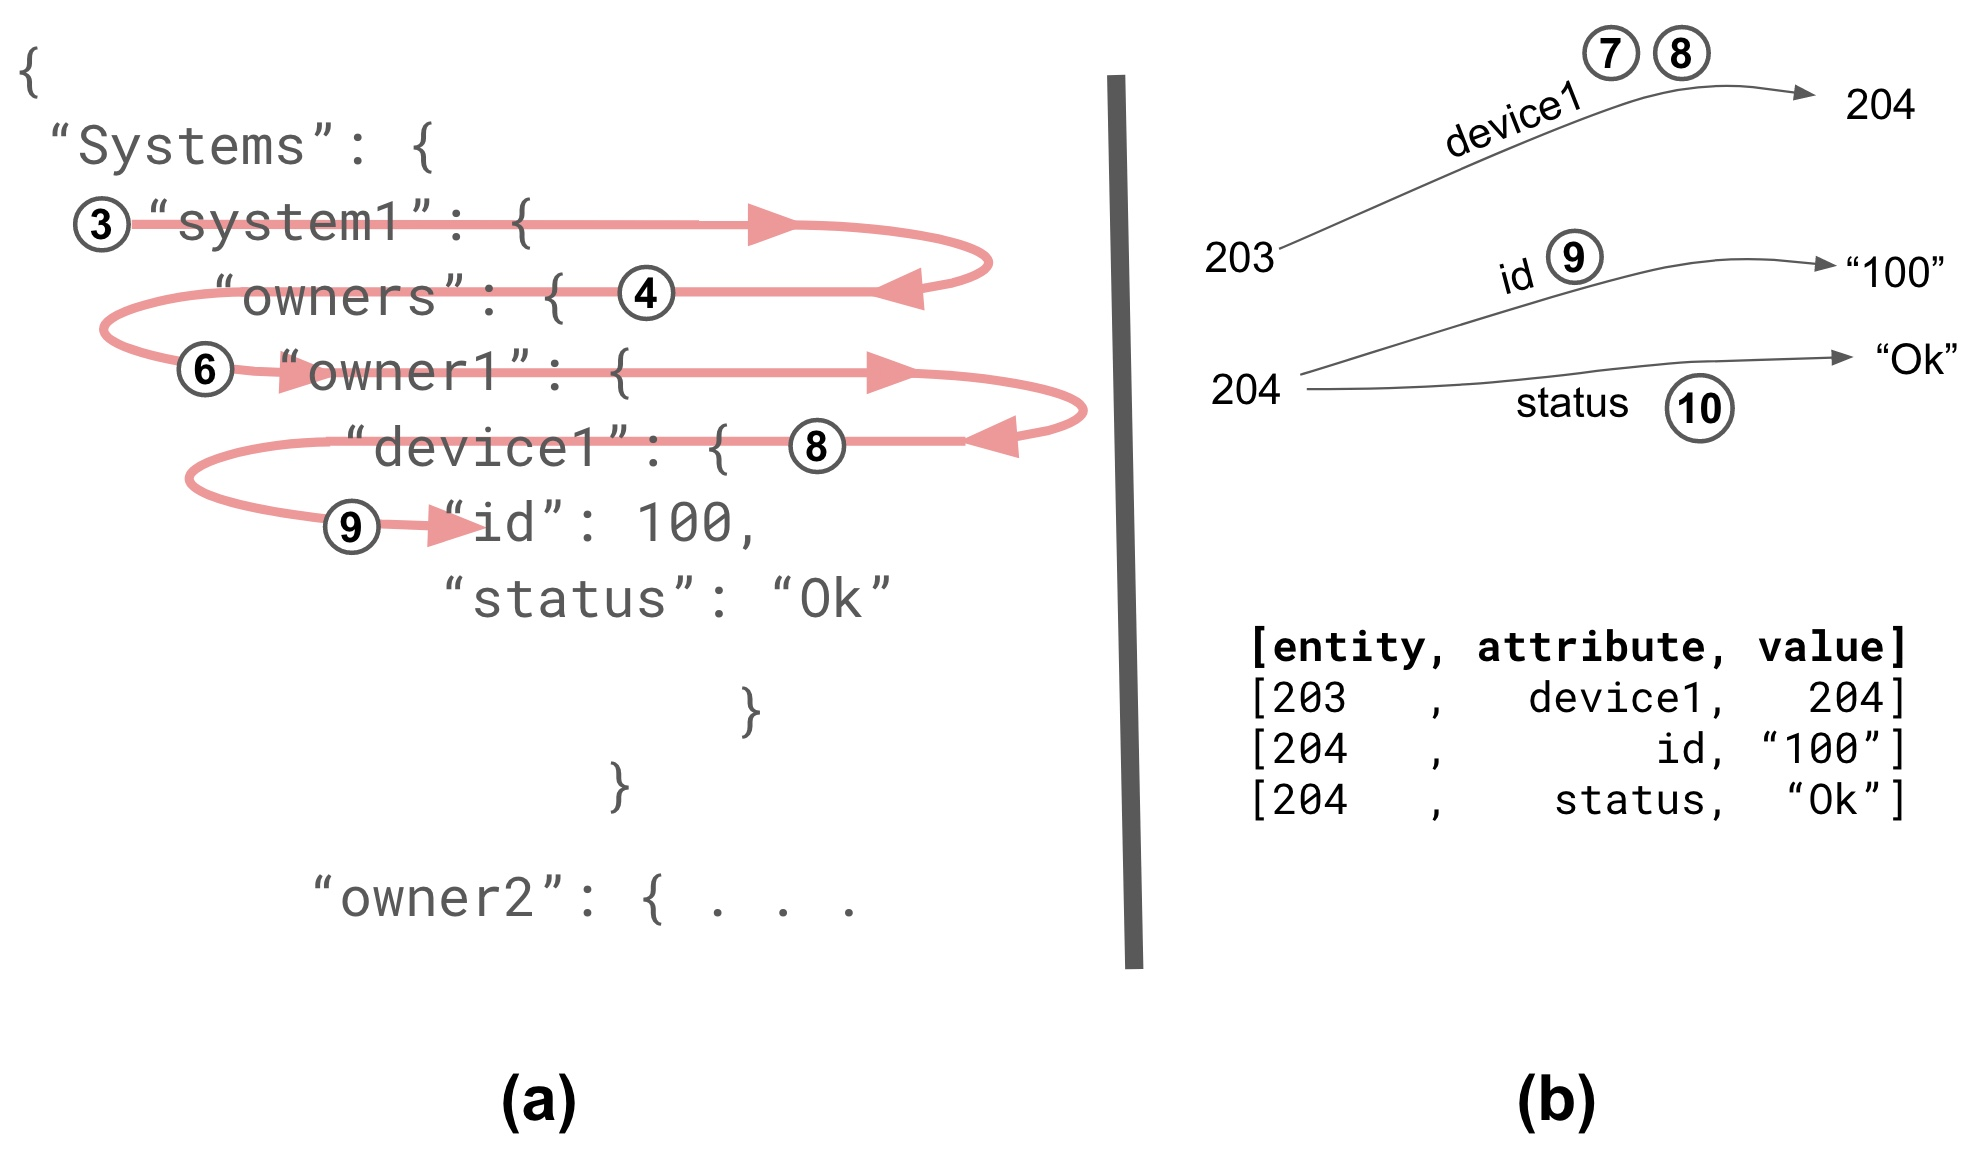
\includegraphics[scale=0.15]{hairpin-two-part.jpg}
  \centering
\end{figure}





%\subsection{Vectors and Iteration}
%
%\subsubsection{Mapping Over a Vector}
%% POD "array" or "collection"?
%In the language, iteration is typically performed implicitly in the sense that when the argument to an operation is an array, the operation is applied to each element of the collection.
%The result returned is an array of the result of applying the operator to each element.
%Thus in Figure~\ref{code:simple-map}, \stt{.zipcode} is applied to the array \stt{\$ADDRS} returning  an array \stt{[``20898'' ``07010-35445'', ``10878'']}.
%
%% https://tex.stackexchange.com/questions/336919/simple-coloring-of-json-attributes
%\lstset{
%%    string=[s]{"}{"},
%%    stringstyle=\color{blue},
%%    comment=[l]{:},
%%    commentstyle=\color{black},
%    basicstyle=\footnotesize\ttfamily
%  }
%
%  % M-x eval-expression (local-unset-key "\"") to work on this! (avoids ``...'').
%\begin{figure}[H]
%\caption{Map over an array of entities, collecting ZIP code.}
% \label{code:simple-map}
%\begin{lstlisting}[language=JavaScript,basicstyle=\ttfamily\scriptsize]
%
%(
%  $ADDRS :=
%     [{"name"     : "Peter",
%       "street"   : "123 Mockingbird Lane",
%       "zipcode"  : "20898"},
%
%       {"name"    : "Bill",
%        "street"  : "23 Main Street",
%        "zipcode" : "07010-3545"},
%
%       {"name"    : "Lisa",
%        "street"  : "903 Forest Road",
%        "zipcode" : "10878"}];
%
%   $ADDRS.zipcode
%)
%
%\end{lstlisting}
%\end{figure}
%
%% I checked: This is what JSONata does too!
%  In the case that the operator returns null for elements of the array, no value is collected.
%  For example, if ``Bill'' in the above didn't have a zipcode, \stt{\$ADDRS.zipcode} would have returned \stt{["20898", "10878"]}.
%
%\subsubsection{Filtering  an Array}
%Suppose, for some odd reason, we didn't like 9-digit Zip codes (what the US Postal Service calls ``Zip+4'') and that we simply want to exclude them from the collection.
%There are a few simple ways to do this.
%One of those is to append a test expression to the end of the previous expression. This ``filtering'' test expression needs to be enclosed in square brackets to indicate that it is filtering.
%\stt{\$ADDRS.zipcode[\$match(/\^{}\textbackslash d[5,5]\$/)]}. Regular expression syntax is arcane but what is shown is typical of JavaScript, Java and many other regex libraries.
%The above matches on strings that are exactly 5 number characters, thus excluding the Zip+4 Zip Codes.
%
%\subsubsection{Index Variables} % Move this to "Challenge problems"???
%Index variables are variables used to iterate through arrays.
%They are common in procedural code, for example, the variable \stt{i} in the pseudocode \stt{for i in [1..9] \{\ldots \}} is an index variable..
%A goal of interoperable exchange is to allow the expression of individual mapping statements that can be defined independent of larger program context.
%This kind of independence is useful in conventional \textit{mapping tables}, spreadsheet used to describe to programmers the intent of proposed mapping.
%The problem with index variables in this regard is that they would add meandering procedural expression where concise, independent, declarative expression is desired.
%%This is why the functional programming features known as \textit{map}, \textit{filter}, and \textit{reduce} are used.
%But what if you needed to enumerate the things you were working with, for example, to put an index number in front of them?
%In cases like this, you can avoid the need for an index variable by using the language's \stt{\$map} higher-order function; it is like JavaScript's \stt{map}.
%See Figure~\ref{code:index-in-map} below.
%
%\begin{figure}[H]
%    \caption{Using an index variable.}
%    \label{code:index-in-map}
%\vspace{3mm}
%    \stt{\$map(\$ADDRS.zipcode, function(\$v, \$i) \{'zip ' \& (\$i+1) \& ' ' \& \$v\})}\\
%\vspace{3mm}
%returns \\
% \stt{[ 'zip 1 20898', 'zip 2 07010-3545', 'zip 3 10878']}.
%\end{figure}
%
%In the above, \stt{function} introduces a function, and the following code in brackets is the body of the function, a single expression is returned.
%In \stt{\$map} (and \stt{\$filter}, and \stt{\$reduce} described later), the function is called once each with each member of the first argument (\stt{\$ADDRS.zipcode} here) in sequence
%as the value bound to \stt{\$v}, and \stt{\$i} is bound in turn to successive integers in the sequence \stt{[1,2,3]}.
%This effectively eliminates the need for user-defined index variables.
%
%\subsection{Working with Code Lists}
%
%A mapping tasks commonly needed is translating a code list, or subsetting one to a set of code values that actually is used in your business processes.
%For example, there is a very large set of codes for transportation events in the code list \textbf{[don't recall the spec]}.
%Suppose you are receiving messages with lots of these values but your order management application only wants to know whether the shipment is likely to be late.
%There is no getting around the fact that you need to explicitly describe a functional relationship to do this; the functional relationship can be implemented as a lookup table.
%The language defines a switch statement to do this kind of thing.
%An example is shown in Figure~\ref{code:mapping-codes}.
%
%\begin{figure}[H]
%    \caption{Mapping code values.}
%    \label{code:mapping-codes}
%%\lstset{frame=tb,numberstyle=\scriptsize,basicstyle=\ttfamily\scriptsize,numbers=left,stepnumber=1,breaklines=true}
%\begin{lstlisting}[language=JavaScript,numberstyle=\scriptsize,basicstyle=\ttfamily\scriptsize,numbers=left,stepnumber=1,breaklines=true]
%  $Codes2OurCodes := function($theirs)
%   {switch $theirs {
%       #{2, 5, 52, 66} : 'late';
%       #{3, 6, 77, 85} : 'on time';
%       * : 'unknown'}
%   };
%\end{lstlisting}
%\end{figure}
%
%The code in Lines 3 and 4 of Figure~\ref{code:mapping-codes} implement a table.
%The \#\{\ldots\} syntax defines sets.
%On Line 3 the source defines set of code values (2, 5, 52, and 66) and its use indicates that elements of this set are mapped to the target value ``late''.
%
%Were the table to be larger, writing it could get tedious.
%For this reason, it might be reasonable to provide an alternative, whereby a lookup table provided elsewhere is referenced.\footnote{The code in Figure~\ref{code:mapping-codes} also
%  shows how names are associated with functions.
%  Functions in the language do not have names.
%  If you need to use a function in multiple places, assign it to a variable as shown in the figure, (use of \stt{\$Codes2OurCodes}).}

\subsection{Working with Tabular Data}

Being able to read  and write spreadsheet information is a very handy capability in mapping.
Of course, Excel-like spreadsheets can have multiple sheets and the content can be non-uniform, including merged cells and formula.
The language currently does not provide means to deal with these complexities.
However simple tables with no surprises and a header row naming columns (and common-separated value (CSV) files that conform to these requirements) can easily be viewed as an array of map structures.
For example, Table~\ref{table:simple} can be viewed as the structure shown in Figure~\ref{code:simple}.

\begin{table}[H]
  \caption{A simple table oriented such that columns name properties.}
\label{table:simple}
\begin{tabular}{r | l | c | l}

\textbf{ShipDate}& \textbf{Item}& \textbf{Qty}& \textbf{UnitPrice} \\ \hhline{=|=|=|=}
        6/15/21	      & Widget 123   &	1	   &  \$10.50 \\
        6/15/21	      & Gadget 234   &	2	   &  \$12.80 \\
        6/15/21	      & Foobar 344   &	1	   &  \$100.00
\end{tabular}
\end{table}

\begin{figure}[H]
    \caption{Table~\ref{table:simple} viewed as an array of map structures.}
    \label{code:simple}
\begin{lstlisting}[language=JavaScript]

[{"ShipDate":  "2021-06-15", "Item":  "Widget 123", "Qty": 1.0, "UnitPrice": 10.5},
 {"ShipDate":  "2021-06-15", "Item":  "Gadget 234", "Qty": 2.0, "UnitPrice": 12.8},
 {"ShipDate":  "2021-06-15", "Item":  "Foobar 344", "Qty": 1.0, "UnitPrice": 100.0}]
\end{lstlisting}
\end{figure}

The built-in function \stt{\$readSpreadsheet} reads spreadsheets.
An example usage is:\\
\vspace{3mm}
\stt{\$readSpreadsheet("data/spreadsheets/ExampleInvoiceInfo.xlsx", "Sales Info")} \\
\vspace{3mm}
where the first argument names an Excel file and the second names a sheet in that spreadsheet.
If the table is transposed (so that all the properties are in its first column, and each row concerns a different object), a third argument with value \stt{true} can be specified to access the data in the more useful orientation.

\section{Working with Data Having Complex Interrelations}
%[This section will introduce provisions for expressing maps to/from relational DBs, where schema are assumed.]

Some situations call for more complex query and restructuring functionality than what has been illustrated above.
Everything to this point in the discussion could be performed easily with JSONata~\cite{Jsonata.org2021}, a language for querying and restructuring JSON-like data.
JSONata is used, for example, in the Open Integration Hub~\cite{OIH2021}, an open software platform that received its initial funding in 2017 from the German Federal Government,
Federal Ministry for Economic Affairs and Energy. % https://www.elastic.io/pressroom/open-integration-hub-data-synchronisation/
JSONata is also used in Node-RED~\cite{Node-Red2021}.

The JSONata viewpoint could be described as one where a tree (or equivalently, a JSON object) is navigated from the root.
Decades of experience, dating back to the early days of EDI, has shown that tree-based organization such as JSON objects is a quite reasonable choice where the communication of document-like information (e.g. ``messaging'') is needed.
The point of an interoperable exchange form such as RADmapper\footnote{RADmapper is my shot at a name. RAD=rapid application development. Suggest a name!}, however, includes additional requirements.
Among these is the ability to describe relationships to and from data possessing complex interrelationship, for example, data described by a relational schema or knowledge graph.
To argue that APIs to the back-end system already do this work is to miss the point:
we are not trying to replace a back-end system function, but to describe the relationships in ways that help business analysts, programmers, and machine agents.\footnote{Likewise we are going to try to address
  situations where there are multiple sources. There are tools to do this already, but again, we are trying to describe the relationships, not replace existing software.}

%========================================================
%  Picture here of navigating a tree versus jumping around to find things in a network.
%========================================================

To illustrate the challenge of using a JSONata-like engine for data having complex interrelations, suppose, for example\ldots. [Discussion of the OWL example]

\subsection{Data Organized as Triples}
Relational and graph-based data can be described by triples $[x,rel,y]$ where $x$ is an entity identifier, $y$ is data (string, number, object, array, another entity identifier, etc.)\footnote{What  additional atomic data
  types shall we provide? Dates? URIs? UUIDs? etc.}~\footnote{Triples provide 5th-normal form relational data. Recomposing a concept from 5-th normal form typically requires as many joins as
  there are attributes to recompose.
  The upside of using triples are that
  (1) substantial amounts of data are already in triples (e.g. RDF etc.),
  (2) some query engines helpfully index triples in multiple ways entity-attribute-value, attribute-entity-value, and attribute-value-entity, and
  (3) mapping engines can use triples effectively.
  The challenge in using triples with this language is in preserving the abstraction of a functional pipeline owed to JSONata-like language features.}
and $rel$ is a relationship (predicate) holding between $x$ and $y$.
The graph-based viewpoint on such data is that $x$ and $y$ are vertices, and $rel$ is an edge.
$rel$ might be implemented as a string.
Thus, the translation of structured data such as JSON objects into such triples is relatively straightforward:
\begin{enumerate}
\item A unique entity identifier is associated with each object; this identifier serves as the first element of triples about that object.
      In JSON, for example, an object is a collection of name-value pairs delimited by curly brackets.
\item Each object attribute is represented by the string naming it\footnote{I suppose we'll only support strings, though namespaced symbols would be nice!}; these supply the second element of the triple, the $rel$.
\item The third element of the triple provides an atomic datum (string, number, entity identifier, etc.) associated with the subject attribute of the subject object.
\end{enumerate}

For example, the first object in Figure~\ref{code:simple}, \stt{\{"ShipDate":  "2021-06-15", "Item":  "Widget 123", "Qty": 1.0, "UnitPrice": 10.5\}} can be encoded as
the following four triples, where the integer 11 is the unique entity identifier for this object.

\begin{lstlisting}[language=JavaScript,basicstyle=\ttfamily\scriptsize]
 [11, "ShipDate",  "2021-06-15"]
 [11, "Item",  "Widget 123"]
 [11, "Qty", 1.0,]
 [11, "UnitPrice", 10.5]
\end{lstlisting}

Of course, an object can have multiple values for an attribute.
For example, a person can have multiple phone numbers.
The way you'd typically handle cardinality greater than 1 in JSON and similar schemes is to simply provide the attribute with an array value.
For example,

\begin{lstlisting}[language=JavaScript,basicstyle=\ttfamily\scriptsize]
 {"name" : "Bob", "phoneNumbers" : ["123-456-1111", "123-456-2222"]}
\end{lstlisting}

In these cases, there would be a triple for each of phone numbers.
Thus, the above might be normalized to triples as follows:

\begin{lstlisting}[language=JavaScript,basicstyle=\ttfamily\scriptsize]
 [12, "name" "Bob"]
 [12, "phoneNumbers" "123-456-1111"]
 [12, "phoneNumbers" "123-456-2222"]
\end{lstlisting}

In the following, an array of objects is used for phone numbers.
Consequently, the \stt{PhoneNumberObjs} triples on entity 13 reference additional entities, not data.

% This is kind of a screwed up example. There should be {phone/type: "cell", phone/num: "123-455-3424"}
\begin{lstlisting}[language=JavaScript,basicstyle=\ttfamily\scriptsize]
{"name" : "Bob", "phoneNumberObjs" : [{"cell" : "123-456-1111"}, {"work" : "123-456-2222"}]}
\end{lstlisting}

\begin{figure}[H]
  \caption{The object for Bob as triples}
  \label{code:bob-phone}
%\lstset{numberstyle=\scriptsize,basicstyle=\ttfamily\scriptsize,numbers=left,stepnumber=1,breaklines=true}
\begin{lstlisting}[language=JavaScript,numberstyle=\scriptsize,basicstyle=\ttfamily\scriptsize,numbers=left,stepnumber=1,breaklines=true]
 [13, "name" "Bob"]
 [13, "phoneNumberObjs" 14]
 [13, "phoneNumberObjs" 15]
 [14, "cell" "123-456-1111"]
 [15, "work" "123-456-2222"].
\end{lstlisting}
\end{figure}

It is worth taking the time to get comfortable with this idea of encoding information in triples;
it is how we work with complex data in RADmapper.


\subsection{Queries on Triples}
You can query triples using Datalog-like notation.\footnote{There are many implementations of Datalog, includes ones for Java and JavaScript, so what is being proposed here should not be hard to implement.} Queries have a square-bracket notation similar to triples illustrated above, but with \textit{query variables} substituted for some of the values.
In JSONata, variables start with a \stt{\$}, in queries, query variables start with a \stt{?}.
For example, \stt{[?e "name" "Bob"]} is a query that will bind the query variable \stt{?e} to the entity identifier of any entity that has "Bob" as its \stt{name} attribute.
But why would you want the entity identifier, it isn't domain data?
The typical answer is that you will need it to perform a sort of join on triples.
For example, if we want to get the \stt{cell} number for \stt{Bob}, we could use the following interrelation of triples.

\begin{lstlisting}[language=JavaScript,basicstyle=\ttfamily\scriptsize]
 [?e "name" "Bob"]
 [?e "phoneNumberObj" ?pn]
 [?pn "cell" ?cellNum]
\end{lstlisting}

If the triples queried are just the ones of Figure~\ref{code:bob-phone}, then the triple on Line 1 matches the query pattern \stt{[?e "name" "Bob"]}, binding \stt{?e} to the entity id 13.
The second query pattern, \stt{[?e "phoneNumberObjs" ?pn]}, matches two triples, those on Lines 2 and 3, binding \stt{?pn} to either entity 14 or 15.
Owing to specifying \stt{"cell"} as the attribute, however, the third query pattern, \stt{[?pn "cell" ?cellNum]}, only matches the triple on Line 4.
This result could be expressed in a JSON-like object notation as a collection of objects such as:
\stt{[\{?e: 13, ?pn: 14, ?cellNum: "123-456-1111"\}]}.
Each such collection of bindings values that together consistently match the query variables in the data is called a \textit{binding set}.
Note that binding sets can contain the database entity IDs, for example, binding \stt{?e} to entity 13 and \stt{?pn} to entity 14 in the above.
Though entity IDs are not part of the domain data, they are part of how data is strung together by the triples and thereby they might be useful.
%For example, the collection of query triples \stt{[?e "name" "Bob"]}, \stt{[?e "phoneNumberObjs" ?pn]}, and
%\stt{[?pn "cell" ?cellNum]} used above could match against various entities where there is an entity whose \stt{name} attribute
%has value "Bob", that entity has a \stt{phoneNumberObj} attribute, and the \stt{?pn} value matches an entity that
%has a \stt{cell} attribute. Each of the binding sets produced would specify values for the three variables \stt{?e}, \stt{?pn} and %\stt{?cellNum}.
Figure~\ref{code:simple-binding-set} depicts another example, the generation of two binding sets from in-line data.

\begin{figure}[H]
  \caption{A simple query against in-line data.}
  \label{code:simple-binding-set}
\begin{lstlisting}[language=JavaScript,numberstyle=\scriptsize,basicstyle=\ttfamily\scriptsize,numbers=left,stepnumber=1,breaklines=true]
  ( $ := [{'Person/firstname' : 'Bob'  , 'Person/lastname' : 'Clark'},
          {'Person/firstname' : 'Peter', 'Person/lastname' : 'Dee'}];
    $.query([?person :Person/firstname ?fname]
             [?person :Person/lastname  ?lname]) )

   /* Returns the following binding set: */
   [{:person 4, :fname 'Peter', :lname 'Dee'}
    {:person 3, :fname 'Bob', :lname 'Clark'}]
\end{lstlisting}
\end{figure}

There are a few thing to note about working with Datalog-like languages like this one.
First, except for performance concerns, it does not matter what order you list the query triples.
Second, you can put query variables in any (or all) of the three positions.
For example, \stt{[?e "cell" "123-456-1111"]} binds \stt{?e} to 14 in the above.
Third, it is possible that there is in the data more than one match;
for example, \stt{[?e ?a ?v]} returns a collection binding set matching all data that is in context.
%It is possible, using query parameters not yet discussed, to limit what is return to the first match, etc.
Finally, you can imagine that using attribute names like "name" and "qty" could get confusing. (Name of what? Quantity of what?)
For this reason, where possible, best practice in Datalog-like languages uses namespaced attributes.
We could use, for example, strings with a slash between the namespace name and the property name.
Thus perhaps, \stt{"Person/name"} and \stt{"Phone/cell"}.
But since these identifiers serve the special purpose of \textit{roles}, the language uses a special syntax: a prefixed colon rather than string delimiters.
Thus \stt{:Person/name} and \stt{:Phone/cell}.
%Where it helps reduce mistakes and the cognitive load on programmers, getting data in that form can be done with JSONata-like pre-processing.
Figure \ref{code:simple-binding-set} above illustrates use of the role syntax on Lines 3 and 4.

\subsection{Query Functions}
%We can now propose a language feature for querying data using the Datalog-like syntax.\footnote{Soon, we will need to demonstrate how this (and the \stt{express} and
%  \stt{transform} language features discussed below) solve problems that are hard to address with strictly JSONata-like capabilities.
%  I'll implement these features and create a Docker web app we can use to play with them. In the mean time, test cases from stakeholders are %\textbf{greatly appreciated!}}

\stt{query} is a RADmapper language element that takes a collection of triple forms and (optional) parameters and returns a function that, when applied to data, returns a collection of binding sets.
For example:

\begin{lstlisting}[language=JavaScript]
 $.query([?e "name" "Bob"]
          [?e "phoneNumberObjs" ?pn]
          [?pn "cell" ?cellNum])
\end{lstlisting}

returns \stt{[\{?e: 13, ?pn: 14, ?cellNum: "123-456-1111"\}]} when \stt{\$} is the data of Figure~\ref{code:bob-phone}.
The example below illustrates the use of an optional parameter \stt{\$name}:

\begin{lstlisting}[language=JavaScript]
 queryCellByName := query($name)([?e "name" $name]
                                   [?e "phoneNumberObjs" ?pn]
                                   [?pn "cell" ?cellNum])
\end{lstlisting}

Using the same data, \stt{\$.queryCellByName("Bob")} would return the same result as the previous query, where "Bob" is hard-coded.

%\footnote{That example uses the JSONata convention that \stt{\$} is the \textit{context reference} always bound to whatever is the data at the time of reference.}
\subsection{Mapping  Networked Data}

Binding sets, in themselves, are not too useful; you might be wondering why we even discuss them.
The answer is that they are crucial to mapping networked data and doing in-place updates.
Once you have the binding sets, you are halfway there; what remains is to use the binding sets to produce target data.
This section describes that process, beginning with definitions of some terms just used:

\begin{description}
\item[networked data] a collection of data that contains pointers to other parts of the same data collection.

  For example, we could have a data in triples that includes information about Bob.
  Instead of repeating everything we know about Bob each time he is referenced in the data,
  networked data can use references to that same data.
  Resolving the reference (which might be implemented as a UUID, for example) connects to the information about Bob.
\item[in-place update] the idea that the mapping task might involve updating an existing collection of data, rather than
  defining new data about it.

  For example, on Bob's 30th birthday, we don't just add the fact \stt{\{'person/name' : 'Bob', 'person/age' : 30\}}, we
  retract the fact that Bob is 29 and assert the new fact.
\end{description}

Before we can talk about mapping networked data and in-place updating, it is important to recognize that these activities require
some additional knowledge about the (target) data.
For example, how do we know
(a) that an action is intended to update some referenced data rather than add new additional information about it, and
(b) whether to use a pointer to reference some data rather than just put the data there?
We need more information about the data.
Specifically, to perform these more complex mapping tasks we have to know:
(1) the cardinality of each attribute,
(2) the type of each attribute (or at least the distinction between references and data types), and
(3) attributes that provide keys (that is, uniquely identify an object of a given type).

% ToDo: This probably belongs somewhere else. (Getting into too much detail!)
Notice that condition (3) mentions the idea of object type.
It is not the case that objects need to have any inherent notion of type to use RADmapper mapping.
It is enough that the programmer recognizes the type by the attributes it possesses.
(This is the so called \textit{duck typing} --- if it walks like a duck and quacks like a duck it is a duck.)
Thus, an object that has an email address and a phone number might be recognized as a customer.
% You already covered this above!
%That said, programmers are likely to have an easier time of it if they explicitly hint at the types of things using namespaced attributes.
%By \textit{namespaced attributes} we mean the idea that the name of the attribute hints at the object type it appears in.
%Thus the attribute for a customers email might be the name-value pair \stt{"customer/email" : "bob@example.com"}.

\subsubsection{Complex mapping task example}

The following example illustrates mapping of a network of Web Ontology Language (OWL) data to a relational form.
The source OWL data used is simplified from actual OWL data to allow easier discussion.
The data consists of objects of two types, one is OWL classes; these have the value  \stt{owl/Class} in their \stt{rdf/type} attribute.
The other is OWL properties (\stt{owl/ObjectProperty}).
The simplifications include using single values for \stt{rdfs/domain}, \stt{rdfs/range}, and \stt{rdfs/subClassOf}.
An OWL class and property is depicted in Figure~\ref{code:endurant}.

\begin{figure}[H]
  \caption{An object (owl/Class) and a relation (owl/ObjectProperty) in the source population.
    These are somewhat simplified from realistic OWL data.}
  \label{code:endurant}
\begin{lstlisting}[numberstyle=\scriptsize,basicstyle=\ttfamily\scriptsize,numbers=left,stepnumber=1,breaklines=true]
{'resource/iri'       : 'dol/endurant',
 'resource/name'      : 'endurant',
 'resource/namespace' : 'dol',
 'rdf/type'           : 'owl/Class',
 'rdfs/comment'       : ['The main characteristic of endurants is...'],
 'rdfs/subClassOf     : :dol/spatio-temporal-particular,
 'owl/disjointWith'   : ['dol/abstract', 'dol/quality', 'dol/perdurant']}

{'resource/iri'       : 'dol/participant',
 'resource/name'      : 'participant',
 'resource/namespace' : 'dol',
 'rdf/type'           : 'owl/ObjectProperty',
 'rdfs/comment'       : ['The immediate relation holding between endurants and perdurants...'],
 'owl/inverseOf'      : 'dol/participant-in',
 'rdfs/domain'        : 'dol/perdurant',
 'rdfs/range'         : 'dol/endurant'}
\end{lstlisting}
\end{figure}

The target data we'll be creating consists of three kinds of things: schema, tables, and columns.
Even with this simple data, there are a few options for designing the relational schema.
The following are design choices that define the form of the mapping target:
\begin{enumerate}
\item Both \stt{owl/Class} and \stt{owl/ObjectProperty} can have \stt{rdfs/comment} and the relationship is one-to-many.
  A single table with keys consisting of the resource IRI and comment text will suffice.

\item \stt{rdf/type} is one-to-one with the class. Though the possible values are limited to just a few such as \stt{owl/Class} and
  \stt{owl/ObjectProperty}, we will represent it with a string naming the type.

\item \stt{resource/name} and \stt{resource/namespace} are also one-to-one and are just the two parts of \stt{resource/iri} and could be computed, but we will store these in the class table too.

\item We will assume \stt{rdfs/domain},  \stt{rdfs/range}, and \stt{rdfs/subClassOf} are single-valued. Typically they are not in a real OWL ontology.

\item We will assume that we want to support storage of individuals of the types defined by OWL classes.
  Though our approach here is not at all reflective of description logic, where class subsumption is the primary kind of inference,
  mapping will produce a two-column table where one column is the individual's IRI and the other is the foreign key of a class to which it belongs.

\item We will assume that all relations are conceptually binary.
  Thus storing individuals means that for each \stt{owl/ObjectProperty} mapping will produce a two-column table to represent both a relation and its inverse (``inverse pairs'') where an inverse is defined.
  Such a table works in both directions (the relation and its inverse), so we will have to prevent creating a table for one member of each inverse pair.

\end{enumerate}

% To keep things simple, we'll omit some otherwise useful considerations like identifying what columns define keys;
%[This belongs elsewhere]: A table keyed by a class \stt{resource/iri} will be defined to store the \stt{resource/name} and \stt{resource/namespace}.
%
With the above considerations in mind, it becomes apparent that some of the work involves nothing more than storing class and property metadata into tables we can define ahead of time.
The \stt{owl/ObjectProperty} definitions, however, entails one new table for each relation (or relation pair if an inverse is defined).
The rows of these tables would be populated by instances of the classes specified by \stt{rdfs/domain} and \stt{rdfs/range}.
This information is not in the ontology, but Figure~\ref{code:static-ddl} depicts the static tables in typical relational DDL.
These are populated by the ontology \stt{owl/Class} content of the
Figure~\ref{code:dynamic-ddl-dml} depicts tables that would be created.

% ToDo: Get listinglst for SQL
\begin{figure}[H]
  \caption{Static DDL for storing class and object relation metadata.
  The mapping will generate information equivalent to DML to populate this from the source data.}
  \label{code:static-ddl}
\begin{lstlisting}[numberstyle=\scriptsize,basicstyle=\ttfamily\scriptsize,numbers=left,stepnumber=1,breaklines=true]
  CREATE SCHEMA typicalOWL;

  CREATE TABLE ObjectDefinition
    (resourceIRI       VARCHAR(300) primary key,
     resourceLabel     VARCHAR(300) not null,
     resourceNamespace VARCHAR(300) not null);

  CREATE TABLE ClassDefinition
    (resourceIRI VARCHAR(300) primary key,
     subClassOf  VARCHAR(300) references ClassDefinition);

  CREATE TABLE ObjectClass
    (resourceIRI VARCHAR(300) primary key,
     class       VARCHAR(300) references ClassDefinition);

  CREATE TABLE DisjointClass
    (disjointID  INT primary key,
     disjoint1   VARCHAR(300) not null references ObjectDefinition,
     disjoint2   VARCHAR(300) not null references ObjectDefinition);

  CREATE TABLE ResourceComment
    (commentID    INT primary key,
     resourceIRI  VARCHAR(300) not null references ObjectDefinition,
     commentText  VARCHAR(900) not null);

  CREATE TABLE PropertyDefinition
    (resourceIRI    VARCHAR(300) primary key,
     relationDomain VARCHAR(300) references ObjectDefinition,
     relationRange  VARCHAR(300) references ObjectDefinition);
\end{lstlisting}
\end{figure}

Figure~\ref{code:dynamic-ddl-dml} depicts the result of mapping data from Figure~\ref{code:endurant} using a mapping
specification that will be described below.

\begin{figure}[H]
  \caption{Result of mapping the data depicted in Figure~\ref{code:endurant}.
    This specifies content equivalent to
    (1) DML to capture metadata for owl/Class and owl/ObjectProperty objects in the static tables defined above, and
    (2) DDL to create tables for owl/ObjectProperty objects.}
  \label{code:dynamic-ddl-dml}
\begin{lstlisting}[language=JavaScript,numberstyle=\scriptsize,basicstyle=\ttfamily\scriptsize,numbers=left,stepnumber=1,breaklines=true]
  {'instance-of'  : 'insert-row',
   'table'        : 'ObjectDefinition',
   'content'      : [{'resourceIRI'       : 'dol/endurant'},
                     {'resourceLabel'     : 'endurant'},
                     {'resourceNamespace' : 'dol'}]}

  {'instance-of'  : 'insert-row',
   'table'        : 'ClassDefinition',
   'content'      : [{'resourceIRI'    : 'dol/endurant'},
                     {'subClassOf'     : 'dol/spatio-temporal-particular'}]}

  {'instance-of'  : 'insert-row',
   'table'        : 'DisjointClass',
   'content'      : [{'disjointID'   ; 1},
                     {'disjoint1'    : 'dol/endurant'},
                     {'disjoint2'    : 'dol/abstract'}]} /* ... (Two more disjoints elided.) */

  {'instance-of'  : 'insert-row',
   'table'        : 'ResourceComment',
   'content'      : [{'commentID'   : 1},
                     {'resourceIRI' : 'dol/endurant'},
                     {'commentText' : 'The main characteristic of endurants is...'}]}

  /* Similar content for the ObjectPropery dol/participant is elided. */

  {'instance-of'  : 'insert-row',
   'table'        : 'PropertyDefinition',
   'content'      : [{'resourceIRI'    : 'dol/participant'},
                     {'relationDomain' : 'dol/perdurant'},
                     {'relationRange'  : 'dol/endurant'}]}

  /* The DDL for the participant table: */

  {'instance-of' : 'create-table',
   'table'       : 'DOLparticipant',
   'columns'     : [{'colName' : 'propertyID',
                     'dtype'   : {'type' : 'varchar', 'size' : 300, 'key' : 'primary'}},
                    {'colName' : 'role1',
                     'dtype'   : {'type' : 'varchar', 'size' : 300, 'ref' : 'ObjectDefinition'}},
                    {'colName' : 'role2',
                     'dtype'   : {'type' : 'varchar', 'size' : 300, 'ref' : 'ObjectDefinition'}}]}
\end{lstlisting}
\end{figure}

%Schema for the target data (the table definitions, etc.) is depicted in Figure ~\ref{code:example-schema-1}.
%The object types define attributes (\stt{db/attrs}) and keys (\stt{db/key}).
%Each attribute has a type (\stt{db/type}) and a cardinality (\stt{db/cardinality}.
%The \stt{db/type} can be any primitive type defined (e.g. strings, numbers, UUID, etc.) or \stt{object}, meaning that
%the attribute is populated by either references to other objects (foreign keys) or objects in-lined in the structure, the choice depending on the value of \stt{db/in-line?}.

%The top-level entries in this schema are identified
%by the strings ``schema'', ``table'', and ``column'' which have no particular significance but might be used in
%error reporting (or we'll get rid of them).

% ToDo: Did I decide to move :db/key ??? If so, do I really need the nested structure?
% ToDo: Do I really want table/schema, or do I want schema/tables?
% \begin{figure}[H]
%   \caption{A schema for the target data}
%   \label{code:example-schema-1}
% \begin{lstlisting}[numberstyle=\scriptsize,basicstyle=\ttfamily\scriptsize,numbers=left,stepnumber=1,breaklines=true]
%   [{'schema' : {'db/attrs'  : [{'schema/name'   : {'db/type' : 'string', 'db/cardinality' : 'one'}}],
%                 'db/key'    : ['schema/name']}}
%
%    {'table'  : {'db/attrs'  : [{'table/name'    : {'db/type' : 'string', 'db/cardinality' : 'one' },
%                                 'table/schema'  : {'db/type' : 'object', 'db/cardinality' : 'one',
%                                                    'db/in-line?' : true},
%                                 'table/columns' : {'db/type' : 'object', 'db/cardinality' : 'many'}}],
%                 'db/key'    : ['table/schema', 'table/name']}}
%
%    {'column' : {'db/attrs'  : [{'column/name'   : {'db/type' : 'string', 'db/cardinality' : 'one'}},
%                                {'column/type'   : {'db/type' : 'string', 'db/cardinality' : 'one'}},
%                                {'column/table'  : {'db/type' : 'object', 'db/cardinality' : 'one'}}],
%                 'db/key'    : ['column/table', 'column/name']}}]
% \end{lstlisting}
% \end{figure}

% The \stt{db/cardinality} of all the attributes in ``one'' except in the case of \stt{table/columns} which is ``many''.
% (See Line 7 of the figure.)
% Cardinality of one means that actions on this attribute of an object necessarily either creates the triple or updates it.
% There will never be two triples about this attribute in the target population where the first two elements of the triple are identical.
% Cardinality of many means that that there could be multiple triples for the attribute.
% Keep in mind that the elements of a triple are always atomic.
% To represent $n$ values there are $n$ triples having different values for the third element of the triple.
% Also, the underlying datalog tool preserves the order of elements in arrays.
%
% Line 7 in the figure demonstrates the use of the optional, \stt{db/in-line?} schema feature.
% On Line7 \stt{db/in-line?} is set to true (the default is false).
% \stt{db/in-line?} true directs the mapper to create structures rather than references.
% Relation technology provides nothing quite like in-lining, but we demonstrate its use in the example below nonetheless.
% In the example, schema are described by just their name; entire objects are serialized like this: \stt{\{schema/name ``some schema''\}}.
% It seems reasonable in these circumstances to in-line, much less so in the case of the back-pointer \stt{table/columns}.

Figure \ref{code:mapping-owl-to-rdbms} depicts the complete specification of a transformation of the source.
\stt{\$transform} is a side-effecting function that takes three arguments, a data context, a binding set, and an express function;
it returns a connection to resulting data.
(Returning the data itself might not be reasonable in the case that it is very large and managed by a database.)
When the binding set argument is a literal call to \stt{query} it is possible for the parser to do syntax checking between
the \stt{query} and \stt{express}.

The \stt{query} produces a binding set for the source data.
The \stt{express} defines how values from the binding set are used in the target population.

% ToDo: Check out the URL about better listing javascript
% https://mysnippets443.wordpress.com/2015/11/28/latex-insert-javascript-code-with-lstlisting-package/

\begin{figure}[H]
  \caption{Mapping the example OWL to the relational database schema}
  \label{code:mapping-owl-to-rdbms}
\begin{lstlisting}[language=JavaScript,numberstyle=\scriptsize,basicstyle=\ttfamily\scriptsize,numbers=left,stepnumber=1,breaklines=true]
  (   $data := $read('data/testing/owl-example.edn');

  $qtype  := query($rdfType, $extraTrips)
               { [?class :rdf/type            $rdfType]
                 [?class :resource/iri        ?class-iri]
                 [?class :resource/namespace  ?class-ns]
                 [?class :resource/name       ?class-name]
                 /* ToDo: $extraTrips */
               };  /* Defines a higher-order function, a template of sorts. */

  $etype  := enforce($tableType)
              {  {'instance-of'  : 'insert-row',
                  'table'        : $tableType,
                  'content'      : {'resourceIRI'       : ?class-iri,
                                    'resourceNamespace' : ?class-ns,
                                    'resourceLabel'     : ?class-name}}
                           }; /* Likewise, for an enforce template. */
                              /* The target tables for objects and relations a very similar. */

  $quClass := $qtype('owl/Class');     /* Use the template, here and the next three assignments. */

  /* This one doesn't just specify a value for $rdfType, but for $extraTrips. */
  $quProp       := $qtype('owl/ObjectProperty'); /* ToDo: ,queryTriples{[?class :rdfs/domain ?domain] [?class :rdfs/range ?range]}); */
  $enClassTable := $etype('ClassDefinition');
  $enPropTable  := $etype('PropertyDefinition');

  /* Run the class query; return a collection of binding sets about classes. */
  $clasBsets := $quClass($data);

  /* We start enforcing with no data, thus the third argument is []. */
  $tar_data := $reduce($clasBsets, $enClassTable, []);

  /* Get bindings sets for the ObjectProperties and make similar tables. */
  $propBsets := $quProp($data);

  /* We pass in the target data created so far. */
  $reduce($propBsets, $enPropTable, $tar_data) /* The code block returns the target data. */
)
\end{lstlisting}
\end{figure}


% $.$transform(
%     query( [?class :rdf/type            'owl/Class']
%             [?class :resource/iri        ?class-iri]
%             [?class :resource/namespace  ?ns]
%             [?class :resource/name       ?class-name]
%             [?rel   :rdfs/domain         ?class-iri]
%             [?rel   :rdf/type            ('owl/ObjectProperty' or 'owl/DataProperty')]
%             [?rel   :rdfs/range          ?rel-range]
%             [?rel   :resource/name       ?rel-name])
%     express( {'table/name'     : ?class-name,
%                'table/schema'   : {'schema/name'  : ?ns},
%                'table/columns'  : {'column/name'  : ?rel-name,
%                                    'column/type'  : ?rel-range,
%                                    'column/table' : ?table-ent}} as ?table-ent))
%
%We'll walk through the example line by line.
%On Line 1 \stt{\$transform} receives data from the context variable. [Other methods will be defined.] % ToDo
%On Line 2 we constrain the search to just those entities that have \stt{rdf/type} containing the string ``owl/Class''.
%On Lines 3, 4, and 5 we bind variables to attribute values of that entity.
%If instead of mapping every namespace in the source data we wanted to limit mapping to a single namespace,
%we could have specified a value or expression for \stt{resource/namespace} on Line 4 rather than the variable \stt{?ns}.
%For example, we could have specified ``dol'' here, that happens to refer to the DOLCE ontology namespace.
%(See the example data in Figure ~\ref{code:endurant}.)
%
%Lines 6, 7, 8 and 9 match and bind a second entity.
%Line 6 uses the variable \stt{?class-iri} which was bound on Line 3; thus a relational join is performed.
%According to Line 7 this entity must have \stt{rdf/type} of either ``owl/ObjectProperty'' or ``owl/DataProperty''.
%Lines 8 and 9 bind the \stt{rdfs/range} and \stt{resource/name} respectively.
%
%With a call to \stt{express}, Line 10 defines  a higher-order function.
%The design of \stt{\$transform}, \stt{query} and \stt{express} were factored as they are to facilitate debugging.
%For example, \stt{query} can be run on context data so that the resulting binding set may be verified;
%\stt{express} can be applied to a small hand-coded binding set to verify that the intended mapping is taking place.
%

% ToDo: This needs work.
The example dataset from DOLCE is fairly large.
Let's suppose it contains 50 classes, each involved in 10 relations.
That suggests a collection of 500 binding sets.
That does not necessarily entail 500 structures like Lines 10 through 14, however.
In contrast to the JSONata-like operations, which maps physical structures to physical structures,
the mapping engine here is mapping between logical structures.
Specifically, a triple represents a fact and the database of triples need only represent a fact once.
It is the knowledge of keys and references provided by the schema that allows the mapping engine to construct physical structure
from the logical relationship defined by the mapping specification.

\subsubsection{Summary of the complex mapping work process}
A good approach to complex mapping tasks might start with performing \stt{query} on the data.

%Since it is likely that we do not have use for the bindings of the entity identifiers bound to \stt{?e} and \stt{?pn}, there is optional syntax in the definition to avoid returning them.
%For example, \stt{queryCellByName := query(\$name)\textbf{(?cellNum)}\{[?e 'name' \$name] \ldots\}} would return a binding set containing %only values for \stt{?cellNum}, if any.

\subsubsection{In-place Updates}

\textbf{[This part needs to be updated.]} Used alone in code, \stt{query} does not fit the pattern of a JSONata-like capability.
JSONata is effective and concise because it allow one to thread data through a pipeline of primitive transformations.
If you place a \stt{query} call anywhere in that pipeline, you lose all the data except what is specifically captured by \stt{query}.
There are certainly instances where that is useful, but is \stt{query} any easier than pure JSONata in these circumstances?\footnote{Stakeholders, do you have
  examples where you think \stt{query} might be better?
  Nothing comes to me, at the moment.
  There is also the matter of getting back an object keyed by binding variables.
  Thus far we haven't defined ways to manipulate that.}
Perhaps the unique value of \stt{query} is as an argument to higher-level functions to do tasks such as in-place and bi-directional updating.
Therefore, discussed next is (1) a new construct called \stt{express} and (2) how \stt{query} and \stt{express} can be used as arguments to a higher-order function \stt{\$transform} to do in-place updating.

\subsection{Working with multiple sources}

\subsection{Working with knowledge graphs}

% [[https://github.com/replikativ/datahike/blob/main/doc/schema.md][Schema-on-read/write discussion]]
%[Describe the need for schemas, data-on-read/data-on-write, etc..]
%[Discuss the use of namespaces.]
%[Discuss what can be done with keys.]

% working with relational data, and exchange forms like EDI requires more functionality.
% The language borrows from QVT-r to achieve these requirements.

\section{Use Cases}

\subsection{Interoperable Mapping Tables}

\subsection{Integration Flows}

\subsection{Data Catalogs and Knowledge Graphs}

\subsection{Data Validation}

\subsection{Joint Cognitive Work / Lo-Code Tools}

\section{Specification}

[This section will include a feature-by-feature description of the language similar to a language reference manual. Right now I've just listed the functions we think are needed.]

\subsection{Language Syntax}
This section is apt to be rewritten several times as the features of the language emerge.

\subsubsection{JSONata Subset}
[I haven't found a formal definition (e.g. BNF) for JSONata, but the following \textit{seems to work}. Not yet complete.]

\begin{Verbatim}[fontsize=\footnotesize]

<content> ::= <code-block> | <exp>

<code-block> ::= '('  (<exp-or-assignment> ';')* ')'

<exp-or-assignment> ::= <exp> | <assignment>

<exp> ::= ( <filter-exp> | <binary-exp> | (<builtin-un-op> <exp>) | <paren-delimited-exp> |
            <square-delimited-exp> |<fn-call> | <literal> | <field> | <id> )
          <conditional-tail>?

<binary-exp> ::= <operand-exp> <binary-op> <exp>

<operand-exp> ::= <field> | <id> | literal | <fn-call> | <delimited> | <unary-op-exp>

<filter-exp> ::=  <operand-exp> '[' <exp> ']'

<conditional-tail> ::= '?'  <exp> ':' <exp>

<range-exp> ::= '[' <exp> '..' <exp> ']'

<fn-call> ::=  <id> '(' (<exp> (, <exp>)*)? ')'

<fn-def> ::= 'function' '(' (<id> (',' <id>)*)? ')' '{' <exp> '}'

<js-map> ::= "{" (<map-pair> (',' <map-pair>)*)? "}"

<map-pair> ::=  <string>" ":" <json-data>

<json-data> ::= STRING | NUMBER | <json-array>

<json-array> :: = '[' (<json-data> (',' <json-data>)*)? ']'

<literal> ::= STRING | NUMBER | 'true' | 'false' | <regex> | <js-map>

<regex> (conforms to JavaScript's implementation)

<id> (a string starting with a \$... More on this later.)

\end{Verbatim}

%\subsection{Table of elementary language features}
%
%\begin{table}[H]
%\begin{tabular}{l | l }
%\textbf{Task}                       & \textbf{Example}       \\ \hhline{=|=}
%Access (or navigate)                & Address.PhoneNumber    \\
%Select from array (simple)          & {[}2{]}                \\
%Select from array (from end)        & {[}-2{]}               \\
%Select all from array               & (done implicitly)      \\
%Select a subset of array            & {[}{[}0..2{]}{]}       \\
%Entire input document               & \$                     \\
%Simple query                        & Phone{[}type='mobile'{]} \\
%Select values of all fields         & Address.*                \\
%Select value from any child         & *.Postcode               \\
%Select arbitrarily deep             & **.Postcode              \\
%Concat                              & 'a' \& 'b'               \\
%Usual numeric operators             &  +,-,*,/                 \\
%Array constructors                  &                          \\
%Object Constructors                 & Phone\{type: number\}    \\
%Object Constructors (force array)   & Phone\{type: number{[}{]}\} \\
%Code Block                          & (exp1; exp2; exp3)          \\
%Value as key in result              & Account.Order.Product\{`Product Name`: Price\} \\
%Map                                 & seq.exp                                        \\
%Filter                              & seq{[}exp{]}                                   \\
%Reduce (group and aggregate)        & seq\{exp:exp, exp:exp…\}                       \\
%Sort                                & seq \textasciicircum (exp)                     \\
%Index                               & seq \# \$var                                   \\
%Join                                & seq @ \$var                                    \\
%Functions (in-line)                 & function(\$x) : \{(…)\};                       \\
%Naming functions                    & $myfunc = function($x)…                        \\
%Context variable                    & \$                                             \\
%Root context variable               & $$                                             \\
%Conditional expression              & pred ? exp : exp                               \\
%Variable binding                    & \$my\_var := "value"                           \\
%Function chaining                   & value $\sim$\textgreater{} $f2 -> $f3          \\
%Regular expressions (like JS)       & /ab123/                                        \\
%Time                                & $now(), $millis()                              \\
%Transform                           & head $\sim$\textgreater | location | update {[},delete{]} |  \\
%Example variable binding            & [needs investigation] \\ %  JSONata  & library.loans@$l.books@$b{[}$l.isbn=$b.isbn{]}.\{ 'title': $b.title, 'customer': $l.customer \}
%Type coersion                       & asType(obj, typespec)                 \\
%Type checking                       & isTypeOf(obj, typespec)               \\
%Coersion to integer                 & toInteger(x)                          \\
%Coersion to real                    & toReal(x)                             \\
%Returning a substring               & substring()
%\end{tabular}
%\end{table}
\bibliography{/Users/pdenno/Documents/bibtex/library}

\end{document}
%%% Local Variables:
%%% mode: latex
%%% TeX-master: "interop-mapping"
%%% End:
